
In the last experiments, after defining all the readout parameters, we have also found the main parameter for qubit control, namely the frequency of the drive pulses.
Now we have to calibrate the drive pulse so that we are able to completely control rotations on the Bloch sphere in $\approx40$ ns~\cite{Rabi1936, Wallraff2005}.

Initially, we focus on calibrating a \pipulse, namely a X gate:
\begin{align*}
    \ket 0 &\xrightarrow{X} \ket 1 \\
    \ket 1 &\xrightarrow{X} \ket 0 \\
\end{align*}
The first elements to reach this control are included in \cref{eq:probability_1}. They will lead us to define:
\begin{itemize}
    \item the amplitude of the \pipulse;
    \item the duration of the \pipulse.
\end{itemize}

Practically, we can do three different, but similar, experiments: rabi-length, rabi-amplitude and rabi-amplitude-length. All these experiments have the same structure:
\begin{itemize}
    \item "Prepare" the qubit in state 0 (usually just waiting for a long enough time);
    \item drive the qubit with a pulse with a specific amplitude and length;
    \item measure;
    \item update the pulse parameter (amplitude, length or both) and iterate;
\end{itemize}

In principle, considering the single-parameter experiments, we expect to see a $\sin^2$ as in \cref{fig:sketch_rabi} and we can select the new parameter value for the \pipulse as half the period.
In this way we are choosing the length and amplitude so that, from the ground-state we can go to the furthest point: the excited state.

\begin{figure}[ht]
    \centering
    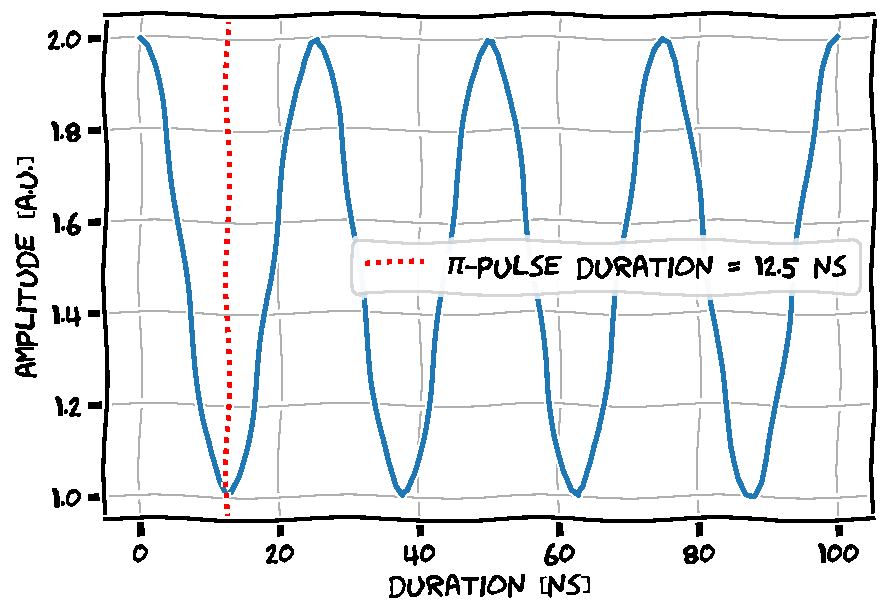
\includegraphics[width=8cm]{characterization/figures/rabi_sketch.pdf}
    \caption{Expected behaviour in Rabi (length) oscillation.}
    \label{fig:sketch_rabi}
\end{figure}

From a practical point of view, however, we still do not have any way of computing \textit{probabilities} and we are just plotting amplitudes: this could lead to deformed curves as, for example, the one plotted in \cref{fig:weird_sketch_rabi}. 
Since we are plotting $AMP=\sqrt{i^2+q^2}$ it can happen that the oscillation between the two center points in the IQ plane does not resembles the expected $\sin^2$.

\begin{figure}[ht]
    \centering
    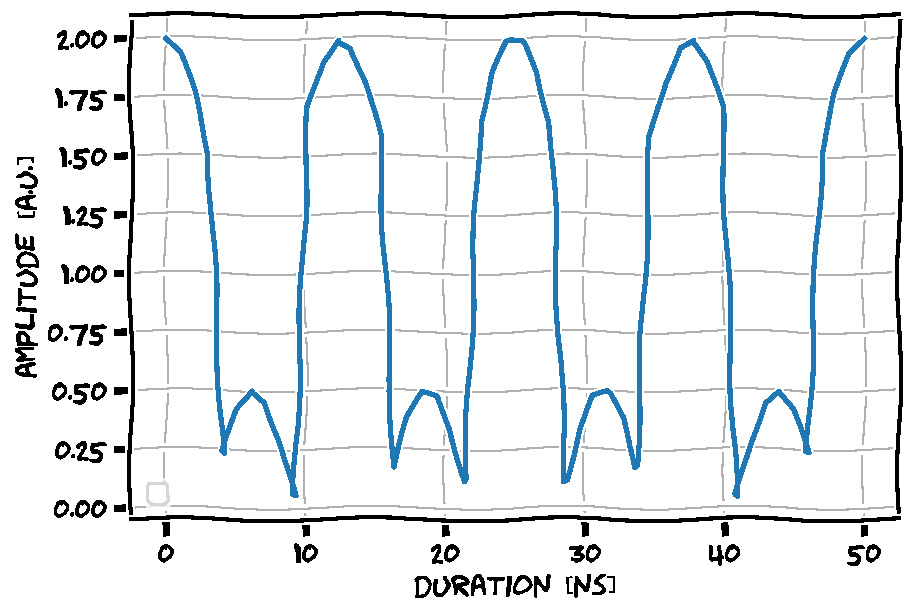
\includegraphics[width=8cm]{characterization/figures/rabi_sketch_problems.pdf}
    \caption{Possible behaviour in Rabi oscillation, when plotting amplitudes.}
    \label{fig:weird_sketch_rabi}
\end{figure}

In any case, we should be able to correctly fit the obtained curve and, eventually, re-do this experiment once we have a way of computing probabilities. Note that the only important parameter here is the period of the oscillation.

For the two-parameters experiment, on the other hand, we expect something like \cref{fig:rabi_amplitude_length}. 
We can see that this plot basically has the two plots combined.

\begin{figure}[ht]
    \centering
    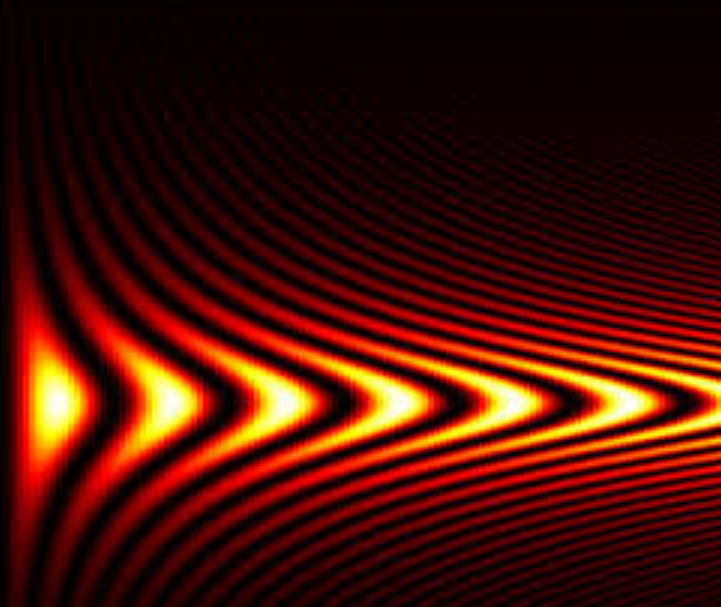
\includegraphics[width=6cm]{characterization/figures/rabi_amplitude_length.png}
    \caption{Plot of a Rabi-amplitude-length oscillations experiment. On the x-axis we have "pulse length", on the y-axis "pulse amplitude".}
    \label{fig:rabi_amplitude_length}
\end{figure}

What are the difference between the three experiment? Should you execute them all?\\
In general, we can avoid to do the two-parameter scan: while it is complete, it is much slower than the single-parameter ones and probes length-amplitude configurations not too useful.
In a practical situation, where no information is given about the qubit, one could simply choose an ansatz on the duration of the pulse: since we want, in the end, fast pulses, a good starting choice could be $40$ ns.
A Rabi amplitude experiment is, usually, more precise than a duration one, but it also more susceptible to range problems: it can indeed happen that the physical range of the DACs is not enough to see a full oscillation.
It is not important to see it, but the fit could be much harder and, in any case, the \pipulse amplitude must be reachable so a new amplificator at the drive line (or less attenuation) could be needed.
Clearly, there is always the possibility to use longer pulses.

On the other hand, Rabi-duration does not incur in these problems, but in general it does not provide the same fine tuning capability.
It can be useful, if we have an idea of the amplitude order of magnitude, to confirm it and to do an estimation of the length.
Moreover, this can help to find the average amplitude for the excited state which we still didn't estimate properly.

In \cref{fig:rabi_length,fig:rabi_amplitude,fig:rabi_amplitude_length}, some plots of the Rabi oscillations experiments are presented.

\begin{figure}[ht]
    \makebox[\textwidth][c]{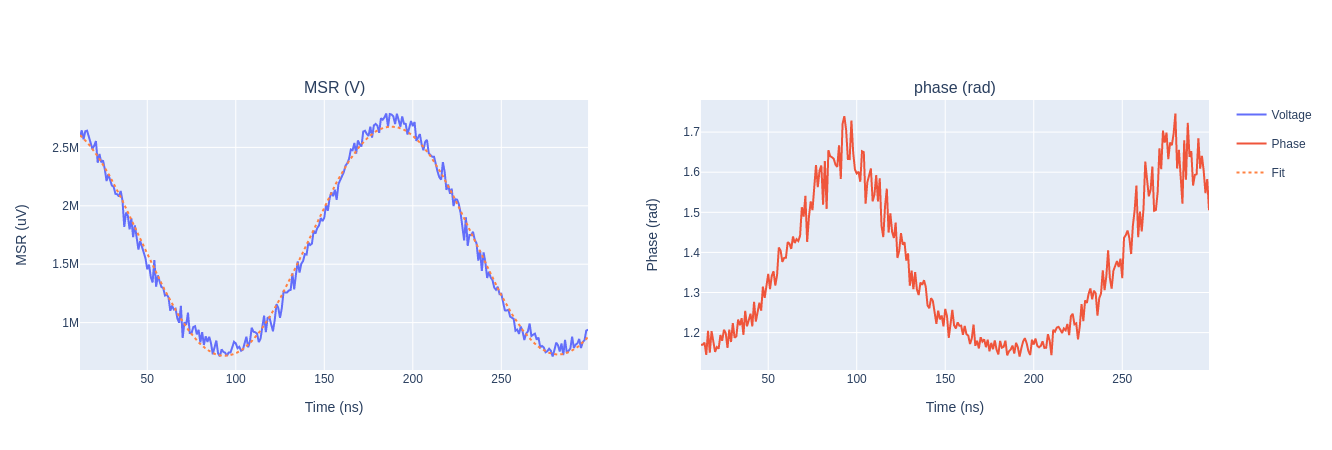
\includegraphics[width=1.3\textwidth]{characterization/figures/rabi_length.png}}
    \caption{Plot of a Rabi-length oscillations experiment.}
    \label{fig:rabi_length}
\end{figure}

\begin{figure}[ht]
    \makebox[\textwidth][c]{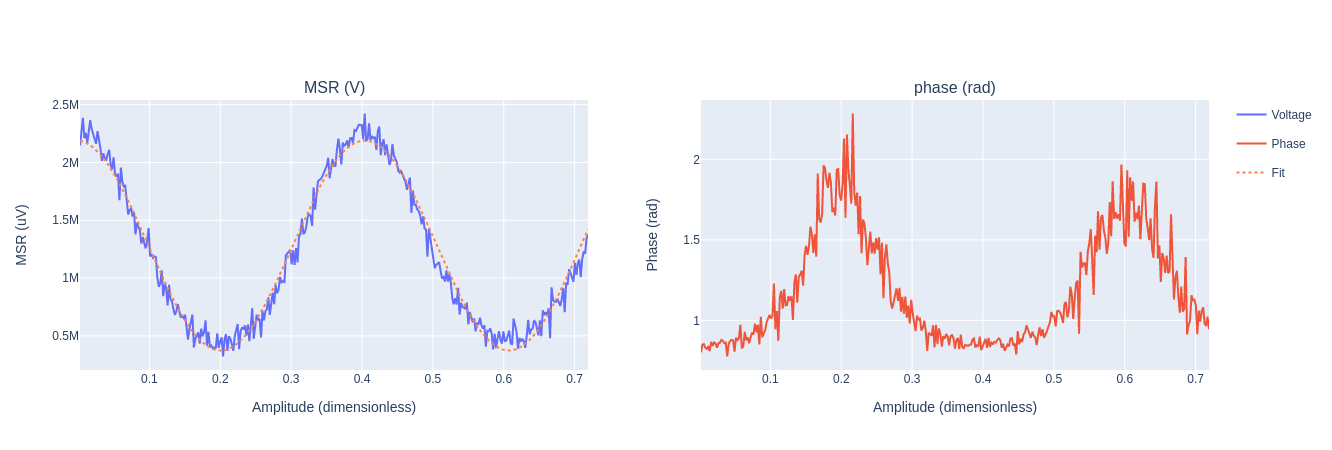
\includegraphics[width=1.3\textwidth]{characterization/figures/rabi_amplitude.png}}
    \caption{Plot of a Rabi-amplitude oscillations experiment.}
    \label{fig:rabi_amplitude}
\end{figure}



In this case, we chose a length of $30$ ns and an amplitude of $0.203$.
In \cref{fig:rabi_amplitude_length} these numbers would describe the shortest central oscillations, nmely the one that maximize the amplitude of the sinusoidal.

\experimentrecap
{Rabi oscillations}
{drive calibration}
{duration of the \pipulse,\\amplitude of the \pipulse,\\estimation of the amplitude relative to the ground and excited state}
{a drive pulse with a specific amplitude and length is sent to the qubit. Afterwards, we perform a measurement of the qubit state. We repeat the experiment for different amplitudes of the drive pulse (or different lengths). We plot the the transmitted/reflected amplitude vs the pulse duration/length. We perform a fit with a $sin^2$, taking half of the period as the \pipulse parameter}


